\chapter{Learning to identify clause types in Mandarin}
\label{chap:man-cl}

In this chapter, we will explore how Mandarin-acquiring children learn clause typing. As we have seen in the last chapter, pragmatic information is crucial for finding the right clause type clustering in English. We found that a learner must have access to some pragmatic information in order to find the right clause types but this learner can succeed with very limited access to pragmatic information. Can we show the same for learners of Mandarin?

As Mandarin [+int] and [imp] have different properties than in English, is it possible for a learner to infer the surface forms associated with these features from the input? Is pragmatics also crucial for Mandarin-acquiring children? And if so, how much pragmatics is required? In this chapter, I address these questions computationally following the same methodology as in Chapter \ref{chap:eng-cl}. I find that, for Mandarin too, surface morpho-syntactic features alone are not sufficient for learners to cluster sentences into the three clause types, so pragmatics is needed. 

This chapter is organized as follows: we will review the properties of Mandarin [+int] and [imp], and children's knowledge regarding these properties. I then report results from a corpus study for Mandarin-speaking parents' input to children in  \ref{sec:mancl:corpus}. The data from the corpus study was used to simulate the two learners, \distlearner{} and \praglearner{}.  %

\section{Background}
\label{sec:mancl:bg}
\subsection{Clause types in Mandarin}
\label{sec:mancl:bg:theory}


In Mandarin, the [+int] value in $C^{0}$ does not trigger movements, but instead shows up in surface form as \twh-phrases, sentence final \tit{ma}, and the A-not-A form. In Mandarin \twh-interrogatives, \twh-phrases  do not need to be fronted to clause-initial position (\citealt{huang1982, cheng1991} among many others). Compare the declarative sentence in (\ref{bg-syn:dec-man}) with the \twh-interrogative in (\ref{bg-syn:wh-man}): the \twh-phrase \tit{shenme} occurs in the same position in the interrogative (\ref{bg-syn:wh-man}) as the noun phrase \tit{zaocan} in (\ref{bg-syn:dec-man}). 


%\begin{minipage}[t]{0.45\linewidth}	
\bex{bg-syn:dec-man}
\gll Xiaoxiao	chi-le zaocan.\\
Xiaoxiao eat-\Asp{} breakfast \\
``Xiaoxiao ate breakfast.''
\eex
\bex{bg-syn:wh-man}
\gll Xiaoxiao	chi-le \tun{shenme}.\\
Xiaoxiao eat-\Asp{} what \\
``What did Xiaoxiao eat?''
\eex


Interrogativity might also have effects on prosody. As mentioned before, \twh-phrases in Mandarin can be interrogative or indefinite (\ref{bg-syn:ambwh}), but interrogative \twh{} is normally associated with prosodic prominence (\cite{hu2002prosody, dong2009, yangyang2018} a.o.).

\bex{bg-syn:ambwh}
\gll Xiaoxiao	mei	chi	\tun{shenme}\\
Xiaoxiao	\Neg{}	eat	what\\
a.	What didn't Xiaoxiao eat?\\
b.	Xiaoxiao didn't eat anything.\\
\eex

\begin{figure}[H]
    \centering
    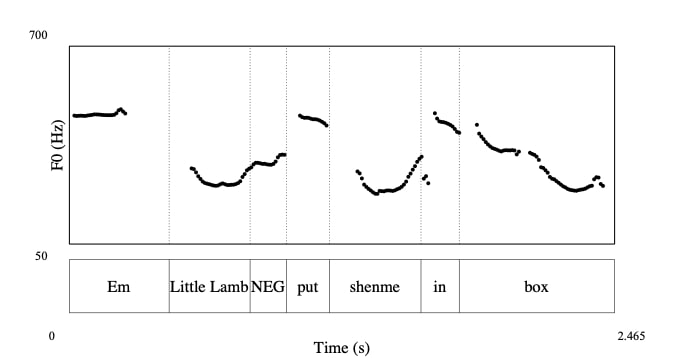
\includegraphics[width=0.6\textwidth]{figures/pitch-FC1wh.jpg}
    \caption{Pitch contour associated with a \twh-interrogative sentence}
    \label{fig:man:wh1}
\end{figure}

\begin{figure}[H]
    \centering
    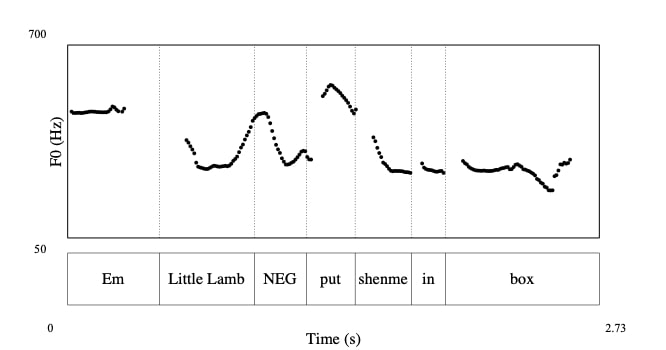
\includegraphics[width=0.6\textwidth]{figures/pitch-FC0wh.jpg}
    \caption{Pitch contour associated with a \twh-indefinite sentence}
    \label{fig:man:wh0}
\end{figure}

 Figure~\ref{fig:man:wh1} shows the pitch contour of the interrogative interpretation of \twh{} and Figure~\ref{fig:man:wh0} shows the indefinite interpretation. The former prosody is associated with [+int] and the latter with [$-$int], and the crucial difference is that the interrogative \tit{shenme} is produced with prosodic prominence (longer duration, extended lexical tone). 

Polar interrogatives in Mandarin also have SVO word order, but are distinguished from declaratives by surface features like the question-forming particle \tit{ma} or the A-not-A construction, as in (\ref{bg-syn:ma}) and (\ref{bg-syn:anota}).

\bex{bg-syn:ma}
\gll Xiaoxiao	chi-le	zaocan		\tun{ma}\\
Xiaoxiao	eat-ASP	breakfast	\Sfp{}\\
``Did Xiaoxiao eat breakfast?''
\eex
\bex{bg-syn:anota}
\gll Xiaoxiao	\tun{chi-mei-chi}	zaocan?\\
	Xiaoxiao	eat-\Neg-eat	breakfast\\
	``Did Xiaoxiao eat breakfast?''
\eex


Sentence final particles (SFPs) like \ma{} are  particles at the right edge of a clause (\citealt{chao1968, zhudexi, huang1982, cheng1991, liboya2006} among others). Many SFPs such as \tit{ba, ya} can occur in any clause type, but \ma{} can only occur in polar interrogatives that do not have the A-not-A form seen in (\ref{bg-syn:anota}). 




To summarize the discussion so far, the surface form of [+int] in Mandarin is sentence final particle \ma{}, A-not-A constructions, and \twh{} with prominence. 

Now, imperatives in Mandarin share many of the properties of imperatives in English, namely the lack of subjects. This clause type is sometimes marked by a negative modal \tit{bie} (and its etymologically related modal \tit{beng}), which only occurs in imperatives (\cite{chao1968, lithompson}):

\bex{ex:man:bie}
\bxl{ex:man:bie:imp}
\gll \tbf{Bie} pao!\\
Don't run\\
``Don't run!''
\ex 
\gll *Zhangsan \tbf{bie} pao.\\
Zhangsan don't run\\
(intended) Zhangsan doesn't run.
\exl
\eex 

Using \tit{bie} as a diagnostic for imperatives, we can see that Mandarin [imp] can be embedded (\cite{lithompson, chen2005imp}), and certain verbs like \tit{zhuzhang} selects [imp]:

\bex{ex:man:embed-imp}
\gll Wo \tun{zhuzhang} Lisi \tbf{bie} chu-guo.\\
I advocate Lisi don't exit-country\\
\trans ``I have the opinion that you don't leave the country.'' \hfill \textcite[p.458]{lithompson}
\eex

While some have argued that certain \Sfp{s} like \tit{ba} are imperative particles (\cite{zhudexi,chao1968,lithompson}), they can actually appear in declaratives, imperatives, and interrogatives, and do not necessarily convey a request/command force (\cite{hanyang1995,liboya2006,ettingermalamud2014,YY2021}):
\bex{ex:mancl:ba}
Xiayu le \tbf{ba}?\\
rain \Asp{} \Sfp{}\\
\trans ``It's raining?''
\eex

Similarly, when these particles append to a declarative clause, they do not change the clause type to [+int]:

\bex{ex:mancl:dec-qa}
\gll %想 坐 啊 ?	Tong
Xiang zuo a?\\
want sit \Sfp{}\\
``Want to sit on it?''
\hfill Declaratives as question\\
Mother of Tong, Session 01;08;22
\eex

The particle \tit{a} elicits a discourse effect along the lines of ``we both know $p$ (or the answers to the question $q$), but let's put it on the table.'' I do not consider this particle to be changing the clause type to be interrogative, just like the final rise in English does not change the clause type of declaratives. This is notwithstanding the fact that the discourse effect of an utterance with \tit{a} is similar to that of a question, namely the speaker wants the addressee to respond. This too is akin to the English final rise.
I therefore do not assume that sentence final particles like \tit{ba} and \tit{a} that can occur across clause types are related to [imp] or [+int].

Thus, [+int] in Mandarin may show up in the surface form of the sentence as the presence of \twh{} with prominence, sentence final \tit{ma}, or A-not-A structure; [imp] shows as sentences without subjects or with second person subjects, and as special negative modal \tit{bie} or \tit{beng} in negative imperatives. 

In sum, Mandarin learners face the same learning problem as English learners: the clause type feature is abstract and is related to a variety of surface forms, none of which is obligatorily present and many of which can occur in sentences with a different clause-type feature on $C^{0}$. Since the surface features indicative of clause type differ between English and Mandarin, however, the problem manifests itself in its own way in each language. For example, even though [imp] is related to null subjects, but since Mandarin is a pro-drop language, it is far more likely that the learner observes a sentence without subject and yet the feature is not [imp].  

\subsection{Mandarin-acquiring children's knowledge of clause types}
\label{sec:mancl:bg:child}
In this section we will look at evidence for Mandarin-acquiring children's knowledge regarding the features reviewed in the last section. For many of these features, we do not have a lot evidence from the comprehension side, and we have to rely on data from children's production alone to make inferences about their knowledge. As production might not be an accurate reflection of children's grammar, we will be conservative in our assessment.   

\tsc{\textpm subjects}   As Mandarin does not have subject-verb agreement, and does not have expletive subjects, it is hard to assess chidlren's knowledge regarding subjecthood. But observations of children's production data before 18 months old suggest that they understand the basic word order of Mandarin as SVO (\cite{tardif1993verb,tardif1996verb}). They also produce subject control sentences (e.g. \tit{Zhangsan tried PRO to help me}) correctly before turning 2 (\cite{yang2015control}). Although this falls out of our interested age range, studies have demonstrated that 2.6-year-olds can correctly distinguish subjects from topics (\cite{chien1985subj}). 

\tsc{\textpm verbs} By 18 months old, Mandarin-acquiring infants produce many verbs, and use verbs productively in many contexts (\cite{tardif1993verb,tardif1996verb, xiaolee2006,zhangshili2015infant}, among many others); while this does not necessarily mean that they have a verb category, it is consistent with the hypothesis that they do . 13-month-olds also demonstrate the ability to categorize novel words as verbs using frequent frames related to verbs, such as auxiliaries (e.g. \tit{bie} ``don't'', \cite{zhang2015bie}) and focus particles (e.g. \tit{ye} ``also'', \cite{zhangshili2015infant}; \cite{ying2021func} for 19-month-olds).

\tsc{\textpm auxiliary}  \cite{zhang2015bie} find that 12-month-olds use functional words to categorize content words, specifically that they could use the negative imperative modal \tit{bie} to identify the follow-up item is a verb, suggesting that children might be sensitive to the presence of this negative modal auxiliary.  %Children are found producing modal auxiliaries like \tit{neng} from 18 months old (\cite{}), but it is unclear whether 


\tsc{\textpm \tit{wh}-phrases} Children start producing interrogative \twh{} as early as 14 months old (\cite{lee1989acq, fan2012, linjing2014}); both comprhension experiments and corpus data show that they are also found to answer \tit{where}, \tit{who}, \tit{what} questions appropriately at 18 months old (\citealt{fan2012,moradlou2020}). While we have evidence that 3-year-olds can use prosodic prominence to infer whether a \twh-sentence is [+int] (\cite{WHanything}), we do not have evidence about younger children. In the corpus study described in the next section, I follow the practice from the last chapter and classify \twh-phrases with focus particles and connectives (e.g. \tit{yaobu} ``if'') as `Unknown Functional Items' (UFI).

\tsc{A-not-A structure} As noted earlier, the A-not-A structure and the presence of sentence-final \tit{ma} both distinguish interrogatives from declaratives in Mandarin. But while there is evidence suggesting that children start producing negation around 1.5 years old (\cite{lee1982neg,fan2007,li2019neg, huang2022manchild} among others), we do not have evidence regarding whether children perceive A-not-A sentences differently from simple negation sentences. Similarly, we do not have evidence regarding whether children treat \tit{ma} differently from sentences with other sentence final particles like \tit{ya}. I therefore simulated a conservative learner who does not have access to A-not-A and \tit{ma} features, and compare it with a knowledgeable learner who does have access to these two features. 





\section{Corpus study}
\label{sec:mancl:corpus}

\subsection{Corpus and methods}
\label{sec:mancl:corpus:method}
For this corpus study, we used data from the Tong subcopora (\cite{TongCorpus}) from CHILDES (\cite{CHILDES}), which contains audio and video recordings of weekly hour-long free play sessions between Tong and his caregivers from 1;7-3;4 in Shenzhen, China where Mandarin is the language of the community. Although this corpus only contains data from one child, it is the source of Mandarin data that is most comparable to the Providence Corpus in terms of the child's age range and availability of audio/video data. If more corpora from Mandarin-speaking children become available in the future, the methodology developed here can be applied to them. Another problem with the corpus is that it does not have data from when before the child was 18 months old, which is older than the age that we assume children figure out the clause type categories; 18 months is also older than the children in the English corpus study. However, while the pragmatics of parent-child interaction might change with children's age, the morpho-syntactic properties of parents' sentences should stay constant. Therefore, we assumed that the input sentences share similar properties as parents' sentences before Tong turns 18 months old. Once corpus data from younger children becomes available, we would apply the same methodology to these data. 

We sampled 500 conversational turns from each session from when the child was 01;07;18 to 2;2;16. Each session was coded by two annotators independently for the Clause Type and Speech Act information (mean cohen's $\kappa$: 0.8). For the morpho-syntactic features, initial annotation was generated by a script (\textcolor{red}{url}) using the morphological tagging provided by the corpus, and then manually corrected. In total, 4501 utterances were annotated. 

\subsubsection{Clause Type}

As in the English corpus study reported in the last chapter, each sentence was annotated with their clause type category, \diis{} (\ref{ex:mancl:annt:cl:dec}-\ref{ex:mancl:annt:cl:imp}). Sentences with only one noun phrase or injectives were annotated as ``fragments'':\footnote{In contrast to English, sentences without verbs might not be fragments in Mandarin, as the copula \tit{shi} ``be'' is optional:
\begin{xlist}
\ex 
\gll Zhe wode.\\
This mine.\\
\trans `This is mine.'
\end{xlist}
}

\bex{ex:mancl:annt:cl}
\bxl \label{ex:mancl:annt:cl:dec}
\gll Wazi shi le.\\
Sock wet \Sfp{}\\
``Your socks got wet.'' \hfill Declarative
\ex \label{ex:mancl:annt:cl:int}
\gll Kandao le ma?\\
See \Asp{} \Sfp{}\\
\trans``Do you see it?''  \hfill Interrogative
\ex \label{ex:mancl:annt:cl:imp}
\gll Gei wo hongse de na-ge.\\
Give me red \tsc{poss} that-\Cl{}\\
\trans``Give me the red one.'' \hfill Imperative
\ex \label{ex:mancl:annt:cl:frag}
\gll Ai-ya!\\
\tsc{intj} \\
\trans ``Wow!'' \hfill Fragments
\exl
\eex

The three major speech acts were also annotated, same as in the English corpus study.

\subsubsection{Morpho-syntactic features for clause typing}

As reviewed in the last section, Mandarin-acquiring children at 18 months old can perceive many morpho-syntactic properties related to clause typing. In particular, they might be able to identify the subject, verb, auxiliary of the sentence, and distinguish functional from lexical items. We additionally adopted the conservative assumption that children at this age might not be able to identify all the \twh-items at this stage, but still assume that they might be able to classify them as functional elements, as they may know the distinction between functional and content elements. We therefore put \twh-items, quantifiers, connectives (e.g. \tit{haishi}, the interrogative ``or''), and focus particles in one category ``unknown functional item (UFI),'' and annotated their position in a sentence: sentence initial, sentence-medial but before the verb, after the verb, or sentence final. In addition to such surface features that were also annotated in the English corpus study, we also annotated for whether the sentence contains an A-not-A structure, and whether there is a sentence-final \tit{ma} particle. But since we do not have evidence for whether children around 18 months can perceive these two cues, as discussed in the last section, when simulating children's learning process, we will compare conservative models without these two cues, and knowledgeable models with these two cues.


Each sentence was annotated with whether or not a surface feature is present. (\ref{ex:mancl:schema:formal:verb})-(\ref{ex:mancl:schema:formal:ma}) demonstrate the surface features we annotated and their examples.  


\begin{exe} \label{ex:mancl:schema:formal:verb}
\ex 
\gll \tbf{kan} zhe-ge.\\
Look this-\Cl{}\\
\trans `Look at this one!'' \hfill +Verb
\end{exe}

\bex{mancl:schema:formal:subj}
\gll \tbf{Wo} zhidao.\\
I know\\
\trans ``I know.'' \hfill +Subject
\eex

\begin{comment}
\bex{mancl:schema:formal:asp}
\bxl
\gll Mama mei gei ni mai \tbf{guo} zhege wanju\\
Mom \Neg{} to you buy \Asp{} this toy\\
\trans`` Mom never bought this toy for you.'' \hfill +Aspect
\exl
\eex
\end{comment}

\bex{mancl:schema:formal:aux}
\bxl
\gll Xiaopengyou bu-\tbf{neng} peng.\\
Children \Neg-can touch\\
\trans ``Children can't touch (this).'' \hfill +Auxiliary
\exl
\eex

\bex{mancl:schema:formal:ufi}
+ Unknown functional items:
\bxl
\gll \tbf{Yaobu} na zhe-ge kapian lai jiao ba\\
%要 不 拿 这 个 卡片 来 教 吧 .
What-if take this-\Cl{} card to teach \Sfp{}\\
\trans ``What if (you) teach with this card.''  \hfill Sentence-initial UFI

\ex
\gll Zheli \tbf{hai} you labi.\\
Here also have crayon\\
\trans ``There's also crayons." \hfill Pre-verbal UFI
\ex
\gll  Limian you \tbf{shenme} ya?\\
Inside have what \Sfp{}\\
\trans ``What's inside?" \hfill Post-verbal UFI
\ex 
\gll Guolai \tbf{ba}\\
Come \Sfp{}\\
\trans ``Come here!'' \hfill Sentence final particle
\exl
\eex

\bex{mancl:schema:formal:anota}
+ A-not-A: 
\bxl
\gll Jintian \tbf{leng-bu-leng} a?\\
Today cold-\Neg-cold \Sfp{}\\
\trans ``Is it cold today?" \hfill \tit{Adj-not-Adj}
\ex 
\gll Ni \tbf{hui-bu-hui} xiezi?\\
You can-\Neg-can write\\
\trans ``Can you write? \hfill \tit{Aux-not-Aux}
\ex \gll Ni \tbf{you-mei-you} xiaoqiche?\\
You have-\Neg-have car\\
\trans ``Do you have cars?'' \hfill \tit{V-not-V}
\ex 
\gll \tbf{Chuan-hao} yifu \tbf{meiyou}?\\
Put-well cloth \Neg{}\\
\trans ``Did you put on your coat?'' \hfill \tit{A-not}
\exl
\eex

\bex{ex:mancl:schema:formal:ma}
\gll Xiayu le \tbf{ma}?\\
Rain \Asp{} \tsc{ma}\\
\trans ``Is it raining?'' \hfill +\tit{ma}
\eex

\subsection{Results}
\label{sec:mancl:corpus:results}

\subsubsection{Overview}
\label{sec:mancl:corpus:results:mapping}

In total, 3077 utterances were annotated. Figure~\ref{fig:man-real-cldist} shows the distribution of clause types in the dataset. As in the English dataset, declarative clauses are the most frequent clause type, followed by interrogatives and imperatives. 

\begin{figure}[H]
    \centering
    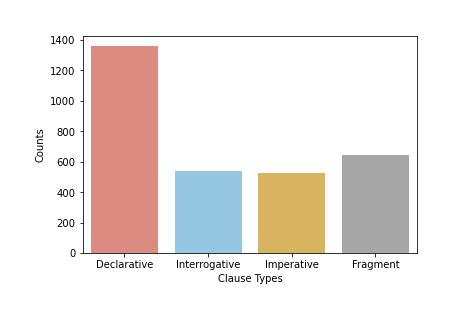
\includegraphics[width=0.7\textwidth]{figures/man-real-cldist.jpg}
    \caption{Distribution of clause types in the corpus}
    \label{fig:man-real-cldist}
\end{figure}

Within interrogatives (Figure~\ref{fig:man:real-subint}), \twh-interrogatives (\ref{ex:man:int:wh}) are more frequent than other types of interrogatives, a pattern similar to the one observed in English; followed by A-not-A (\ref{ex:man:int:anota}) and \tit{ma}-interrogatives (\ref{ex:man:int:ma}). Disjunctive interrogatives with \tit{haishi} ``or'' (\ref{ex:man:int:haishi}) are relatively rare. 
\begin{figure}[H]
    \centering
    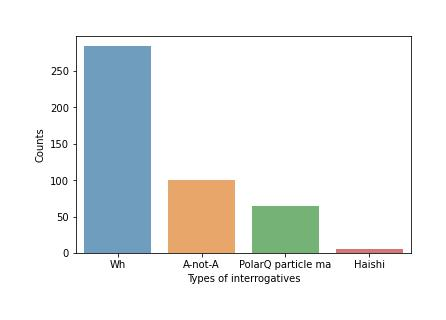
\includegraphics[width=0.7\textwidth]{figures/man-real-subint.jpg}
    \caption{Subcategories of interrogatives}
    \label{fig:man:real-subint}
\end{figure}

\bex{ex:man:int:corpus}
\bxl\label{ex:man:int:wh}
\gll Zhe \tbf{shenme} a?\\
this what \Sfp{}\\
``What is this?'' \hfill  \twh-interrogative\\Mother of Tong, Session 01;10;17
\ex\label{ex:man:int:anota}
\gll Na \tbf{xi-bu-xihuan} he naifen a?\\
Then like-\Neg-like drink {baby formula} \Sfp{}\\
\trans ``Do you like {baby formula} then?'' \hfill A-not-A interrogative\\
Mother of Tong, Session 02;00;19
\ex\label{ex:man:int:ma}
\gll Ni Zhidao \tbf{ma}?\\
You know \tsc{ma}\\
\trans ``Do you know?'' \hfill Ma-interrogative\\Mother of Tong, Session 01;10;17
\ex\label{ex:man:int:haishi}
\gll Qiezi haochi \tbf{haishi} baicai haochi?\\
Eggplant tasty or cabbage tasty\\
\trans ``Is eggplant tastier or cabbage tastier?"\hfill \tit{Haishi} interrogative\\Father of Tong, Session 01;08;22
%茄子 好吃 还 是 白菜 好吃 ? 
\exl
\eex

\begin{figure}[H]
    \centering
    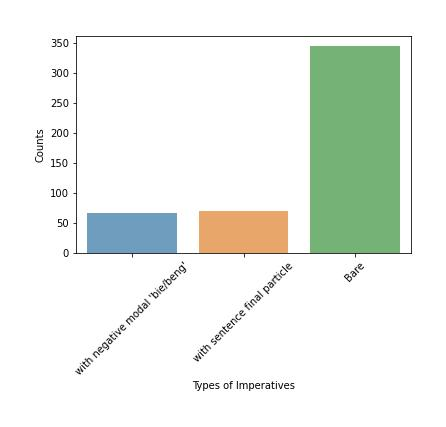
\includegraphics[width=0.7\textwidth]{figures/man-real-subimp.jpg}
    \caption{Subcategories of imperatives}
    \label{fig:man:real-subimp}
\end{figure}

Imperative sentences (Figure~\ref{fig:man:real-subimp}) mostly come without any marker like (\ref{ex:man:impbare}); \tit{bie}-imperatives (\ref{ex:man:impbie}) and SFP-imperatives (\ref{ex:man:impba}) are equally frequent. 

\bex{ex:man:imp:corpus}
\bxl\label{ex:man:impbare}
\gll Kan zhege shi shenme dongxi\\
look this is what thing\\
``See what this is!''  \hfill Imperative (used as a question)\\
Mother of Tong, Session 02;00;19

\ex \label{ex:man:impbie}
\gll \tbf{Bie} fan le!\\
Don't turn \Asp{}\\
``Stop messing around!'' \hfill \tit{Bie}-imperative\\Mother of Tong, Session 02;00;09
\ex \label{ex:man:impba}
\gll Reng zheli \tbf{ba}\\
throw here \Sfp{}\\
\trans ``Throw it here!''
\hfill SFP imperative\\Mother of Tong, Session 02;01;17
\exl
\eex


As for speech acts, Figure~\ref{fig:man-real-sp} shows the distribution of speech acts. Same as in English, assertions are the most frequent speech acts, followed by questions and requests. 
\begin{figure}[H]
    \centering
    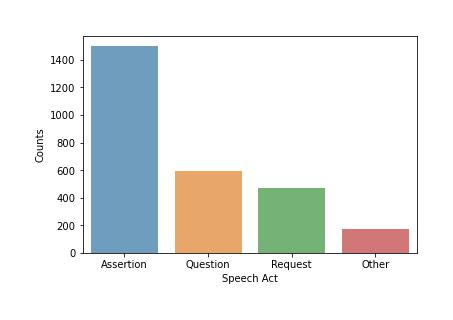
\includegraphics[width=0.7\textwidth]{figures/man-real-sp.jpg}
    \caption{Distribution of speech acts in the corpus}
    \label{fig:man-real-sp}
\end{figure}

The mapping between speech acts and clause types also shows a similar pattern as in English, as illustrated by Figure~\ref{fig:man-real-clsp} and \ref{fig:man-real-spcl}. Declaratives are mostly used as assertions, interrogatives as questions, and imperatives as requests. 

\begin{figure}[H]
    \centering
    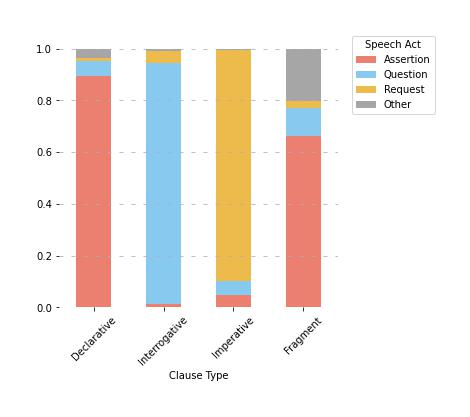
\includegraphics[width=0.7\textwidth]{figures/man-real-clsp.jpg}
    \caption{The speech acts performed by each clause type in parents' speech}
    \label{fig:man-real-clsp}
\end{figure}

\begin{figure}[H]
    \centering
    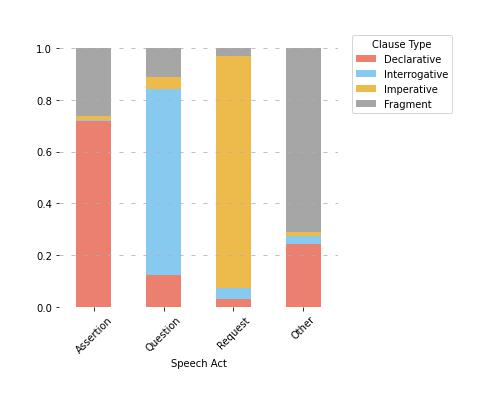
\includegraphics[width=0.7\textwidth]{figures/man-real-spcl.jpg}
    \caption{The clause type used to express each speech act in parents' speech}
    \label{fig:man-real-spcl}
\end{figure}

The proportion of mismatches is small and they form a systematic subcategory. All interrogatives that are used as assertions are rhetorical questions (\ref{ex:mancl:int-asst}). The proportion of interrogatives as requests is smaller than what we observed in the English study (\ref{ex:mancl:int-req}). Even in the small portion of cases we found here, it could be debated whether the non-literal speech act of this sentence is request, as the mother is still asking about the child's ability whereas indirect requests in English like \tit{can you pass the salt} are much more saliently to be interpreted as requests instead of inquiries about the addressee's ability. 

\bex{ex:mancl:int-asst}
\gll Ni xia gaoxing ge shenme ya\\
you blindly happy \Cl{} what \Sfp{}\\
``What are you happy about.'' \hfill Interrogative as question \\
Mother of Tong, Session 02;00;19
%你 瞎 高兴 个 什么 呀 
\eex

\bex{ex:mancl:int-req}
\gll Tongtong hui bei ma?\\
Tongtong can recite \tsc{ma}\\
\trans ``Can you recite (this poem), Tongtong?''
\hfill Interrogative as Requests \\
Mother of Tong, Session 02;00;19
%你 瞎 高兴 个 什么 呀 
\eex

When imperatives are not used as requests, it is almost exclusively with \tit{kan} ``look" and \tit{gaozu} ``tell'':
\bex{ex:mancl:imp-q}
\gll Gaosu mama zhe shi shenme ya?\\
Tell mom this is what \Sfp{}\\
``Tell mom what this is'' \hfill Imperative as question\\
Mother of Tong, Session 02;00;19
\eex

Declaratives as questions often occur with sentence final particles like \tit{a}:
\bex{ex:mancl:dec-q}
\gll %想 坐 啊 ?	Tong
Xiang zuo a?\\
want sit \Sfp{}\\
``Want to sit on it?''
\hfill Declaratives as question\\
Mother of Tong, Session 01;08;22
\eex

As we have discussed, the final particle \tit{a} does not change the clause category of the sentence, but still elicits a discourse effect similar to a question's effect, namely that the speaker wants the addressee to settle an issue.

%%%%%%%%%%%%%%%%%%
\subsubsection{Morpho-syntactic cues}
\label{sec:mancl:corpus:results:syn}


\begin{figure}[H]
    \centering
    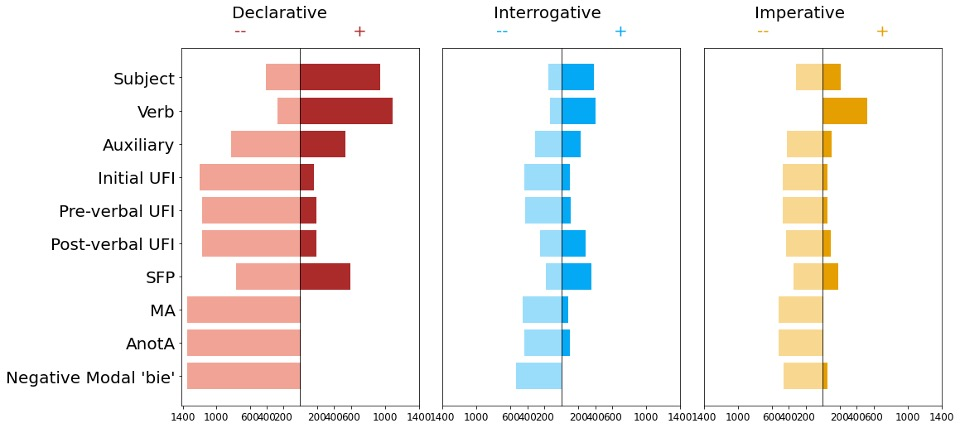
\includegraphics[width=1\textwidth]{figures/man-real-syncluster.jpg}
    \caption{Number of sentences with/without various formal cues in each clause type; darker colors represent number of sentences with the cue, lighter colors, number of sentences without the cue }
    \label{fig:man-real-syncluster}
\end{figure}


%\subsubsection{Informativeness of the cues}
%\label{sec:mancl:corpus:results:supervised}


\section{Modeling the learning of clause type in 
Mandarin}
\label{sec:mancl:model}

In this section, I applied the same Bayesian cluster models as reported in the last chapter to the Mandarin data. As mentioned earlier, we do not have evidence for whether Mandarin-speaking children identify A-not-A constructions or sentence final \tit{ma}. Therefore, I ran two separate simulations for each model (four simulations in total): a conservative learner that do not have access to whether A-not-A or \tit{ma} are present, and a knowledgeable learner that do have access. (\ref{ex:mancl:formal-consornot}) lists the morpho-syntactic cues that each learner have access to.

\bex{ex:mancl:formal-consornot}
For the conservative learner: \\
\textpm subject, \textpm verb, \textpm auxiliary, \textpm sentence-initial UFI, \textpm pre-verbal UFI,  \textpm post-verbal UFI, \textpm sentence final particle
\ex For the knowledgeable learner:
\textpm subject, \textpm verb, \textpm auxiliary, \textpm sentence-initial UFI, \textpm pre-verbal UFI,  \textpm post-verbal UFI, \textpm sentence final particle, \textpm A-not-A, \textpm \tit{ma}
\eex

We used the same methodology and learning models as in the English study in Chapter \ref{chap:eng-cl}. The results are as follows.

\subsection{Performance of the \dlearnerabbr{} model}
\label{sec:mancl:model:results:d}


\subsubsection{The conservative simulation} 
The conservative simulation of the \dlearnerabbr{} model does not use interrogative-specific features \textpm A-not-A construction and \textpm \tit{ma}. From the results, it does not seem like the model identified any meaningful grammatical class in Mandarin.

Figure~\ref{fig:man-baseline-conservative-heat} shows the proportion of \diis{} in each identified cluster, and Figure~\ref{fig:man-baseline-conservative-heatrev} shows the proportion of sentences clustered together. 



\begin{figure}[H]
    \centering
    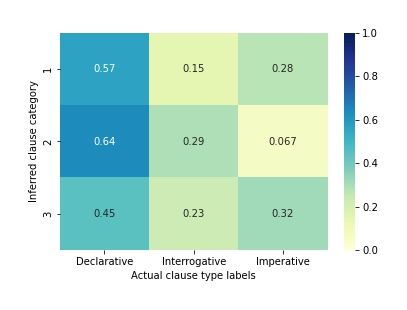
\includegraphics[width=0.7\textwidth]{figures/man-baseline-conservative-heat.jpg}
    \caption{The proportion of \diis{} in each of the three clusters identified by the \dlearnerabbr{} model}
    \label{fig:man-baseline-conservative-heat}
\end{figure}


\begin{figure}[H]
    \centering
    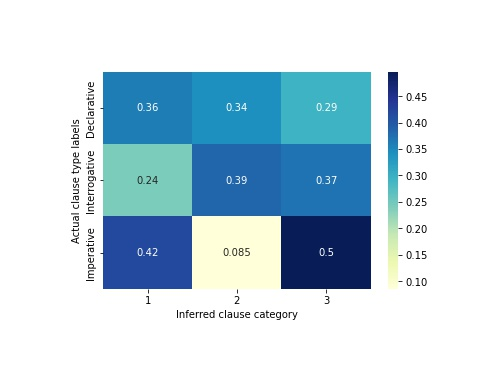
\includegraphics[width=0.7\textwidth]{figures/man-baseline-conservative-heatrev.jpg}
    \caption{The proportion of actual \diis{} clustered in one category}
    \label{fig:man-baseline-conservative-heatrev}
\end{figure}

As we can see, the conservative \dlearnerabbr{} fail to identify any clause types. Each cluster contains all three clause types, and all three clause types are distributed across the three clusters. 

\begin{figure}[H]
    \centering
    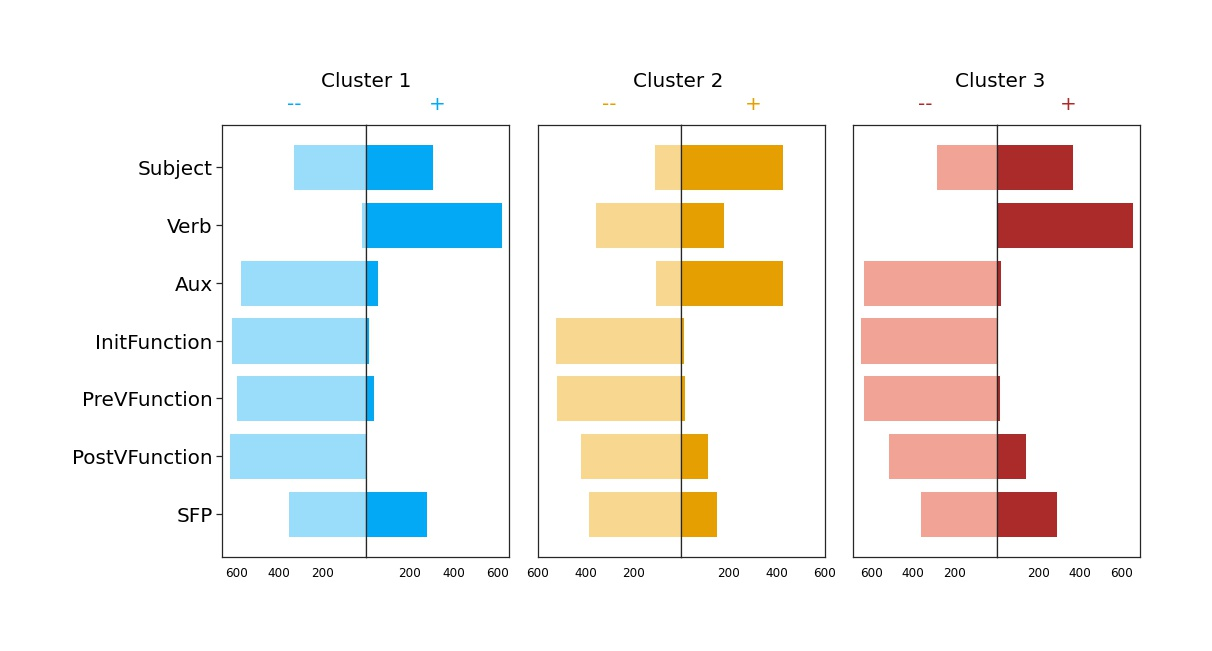
\includegraphics[width=1\textwidth]{figures/man-baseline-conservative-syncluster.jpg}
    \caption{The number of sentences with/without certain formal features in each cluster, darker colors represent the number of sentences with the feature. }
    \label{fig:man-baseline-conservative-syncluster}
\end{figure}

Figure~\ref{fig:man-baseline-conservative-syncluster} shows the distribution of morpho-syntactic features across all three clusters. The three clusters do not seem to form meaningful grammatical classes.

\subsubsection{The knowledgeable simulation}
The knowledgeable simulation of the \dlearnerabbr{} model uses interrogative-specific features, \textpm A-not-A construction and \textpm \tit{ma}. But it also failed to identify any meaningful grammatical class in Mandarin.

\begin{figure}[H]
    \centering
    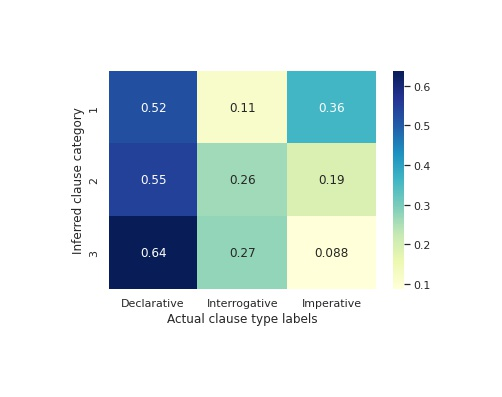
\includegraphics[width=0.7\textwidth]{figures/man-baseline-mid-heat.jpg}
    \caption{The proportion of \diis{} in each of the three clusters identified by the \dlearnerabbr{} model}
    \label{fig:man-baseline-mid-heat}
\end{figure}



\begin{figure}[H]
    \centering
    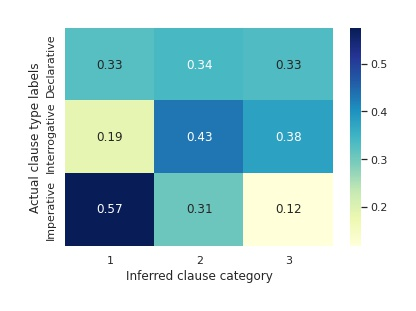
\includegraphics[width=0.7\textwidth]{figures/man-baseline-mid-heatrev.jpg}
    \caption{The proportion of actual \diis{} clustered in one category}
    \label{fig:man-baseline-mid-heatrev}
\end{figure}

Overall, Figure~\ref{fig:man-baseline-mid-heat} shows that all three clusters identified by the \dlearnerabbr{} model are predominantly declarative sentences, which simply reflects the fact that declaratives are the most frequent clause type in the dataset. But compared to the conservative simulation, it puts more interrogatives in Cluster~$2$, as shown in Figure~\ref{fig:man-baseline-mid-heatrev}. But a closer look at the distribution of morpho-syntactic cues within each cluster (Figure~\ref{fig:man-baseline-syncluster} suggests that none of the clusters are meaningful grammatical classes in Mandarin. %The only recognizable feature considers Cluster~$2$ a cluster that allows sentence final particles, which does not correspond to any sentence types in Mandarin.  

\begin{figure}[H]
    \centering
    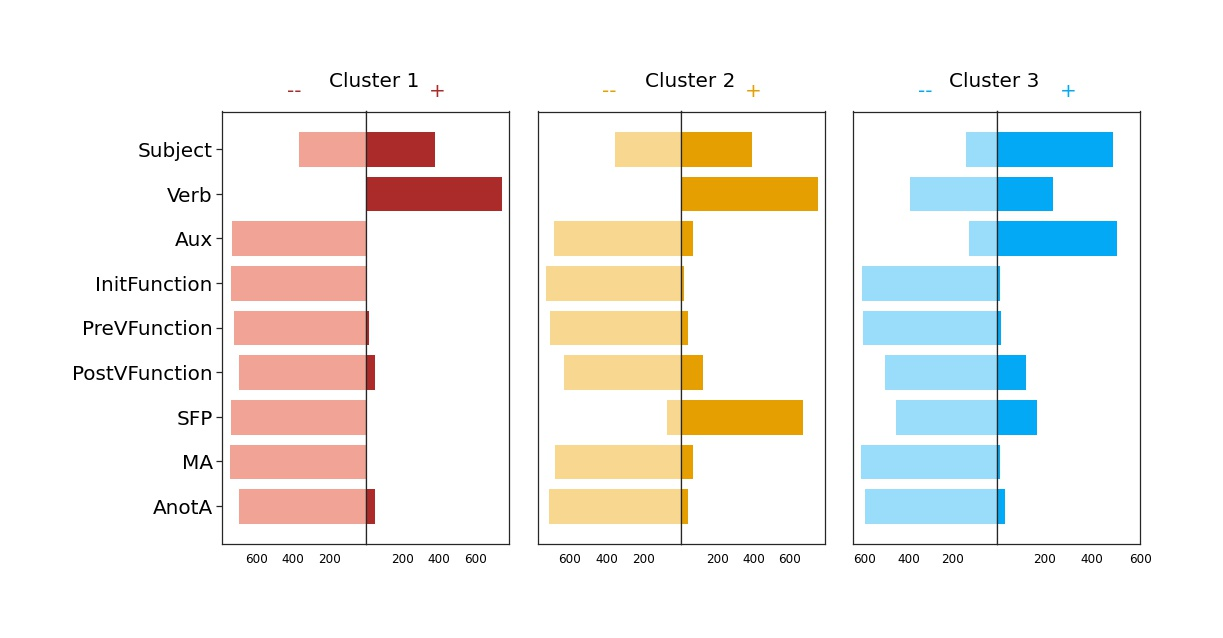
\includegraphics[width=1\textwidth]{figures/man-baseline-mid-syncluster.jpg}
    \caption{The number of sentences with/without certain formal features in each cluster, darker colors represent the number of sentences with the feature. }
    \label{fig:man-baseline-syncluster}
\end{figure}


These results suggest that regardless of whether the model has access to interrogative-specific features or not, the \dlearnerabbr{} failed to identify any of the clause types. It failed to find any meaning grammatical classes. 



\subsection{Performance of the \plearnerabbr{} model}
\label{sec:mancl:model:results:p}
\subsubsection{The conservative simulation}
By having access to pragmatic information, the conservative \plearnerabbr{} model could identify two clause types. Figure~\ref{fig:man-target-conservative-heatmap} shows the proportion of \diis{} in each identified cluster, and Figure~\ref{fig:man-target-conservative-heatrev} shows the proportion of sentences clustered together. 

\begin{figure}[H]
    \centering
    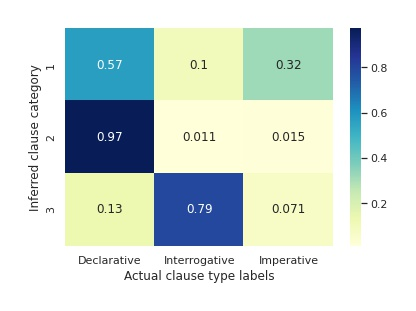
\includegraphics[width=0.7\textwidth]{figures/man-target-conservative-heatmap.jpg}
    \caption{The proportion of \diis{} in each of the three clusters identified by the \plearnerabbr{} model}
    \label{fig:man-target-conservative-heatmap}
\end{figure}




\begin{figure}[H]
    \centering
    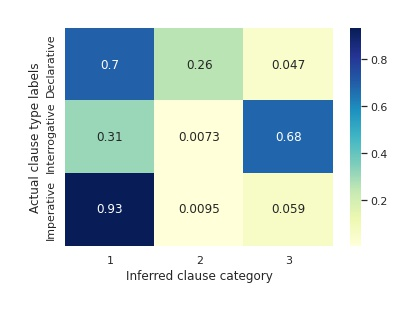
\includegraphics[width=0.7\textwidth]{figures/man-target-conservative-heatrev.jpg}
    \caption{The proportion of actual \diis{} clustered in one category}
    \label{fig:man-target-conservative-heatrev}
\end{figure}


We can see that the \plearnerabbr{} model clearly identifies a declarative and an interrogative cluster: 97\% of Cluster~$1$ are declaratives, 79\% of Cluster~$3$ are interrogatives. Declaratives and interrogatives in Mandarin are also mostly clustered together by the model: 70\% of declaratives, 90\% of interrogatives, and 93\% of imperatives are clustered together in Cluster~$1$, $3$, $1$ respectively. In contrast to \dlearnerabbr{}, this learner is able to find at least one clause type in Mandarin.


Figure~\ref{fig:man-target-conservative-syncluster} shows the morpho-syntactic profile of each cluster identified by the \plearnerabbr{}. 

\begin{figure}[H]
    \centering
    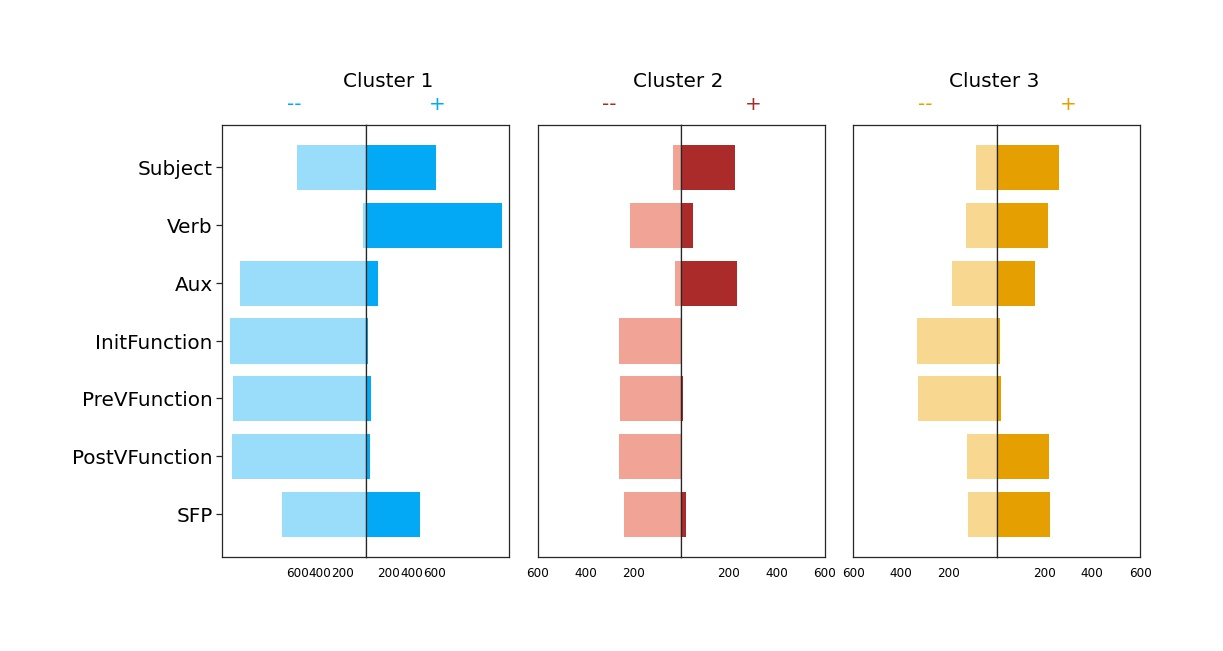
\includegraphics[width=1\textwidth]{figures/man-target-conservative-syncluster.jpg}
    \caption{The number of sentences with/without a formal property in each cluster (Cluster 1 $\sim$ imperatives, Cluster 2 $\sim$ declaratives, Cluster 3 $\sim$ interrogatives), darker colors represent the number of sentences with the property, lighter colors represent sentences without the property.}
    \label{fig:man-target-conservative-syncluster}
\end{figure}

\subsubsection{The knowledgeable simulation}
By having access to pragmatic information, the knowledgable \plearnerabbr{} model could identify two clause types, one for interrogatives and one for declaratives, but imperatives and declaratives are still collapsed into one cluster. Figure~\ref{fig:man-target-mid-heatmap} shows the proportion of \diis{} in each identified cluster, and Figure~\ref{fig:man-target-mid-heatrev} shows the proportion of sentences clustered together. 

\begin{figure}[H]
    \centering
    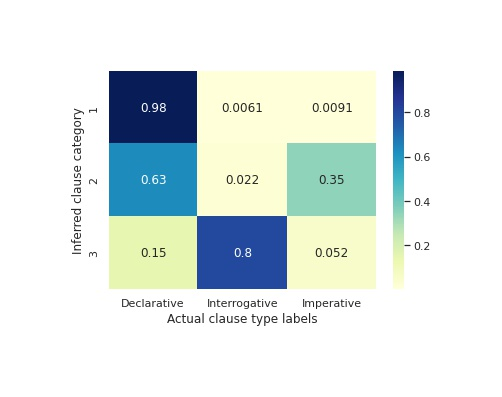
\includegraphics[width=0.7\textwidth]{figures/man-target-mid-heatmap.jpg}
    \caption{The proportion of \diis{} in each of the three clusters identified by the \plearnerabbr{} model}
    \label{fig:man-target-mid-heatmap}
\end{figure}




\begin{figure}[H]
    \centering
    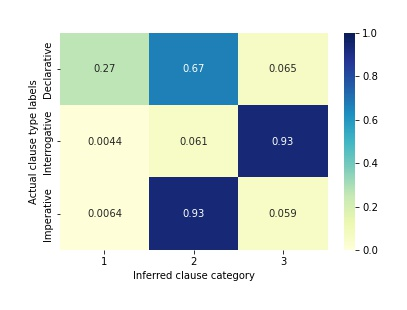
\includegraphics[width=0.7\textwidth]{figures/man-target-mid-heatrev.jpg}
    \caption{The proportion of actual \diis{} clustered in one category}
    \label{fig:man-target-mid-heatrev}
\end{figure}


The \plearnerabbr{} model identifies a declarative and an interrogative cluster: 98\% of Cluster~$1$ are declaratives, 80\% of Cluster~$3$ are interrogatives. The three clause types are also mostly clustered together by the model: 67\% of declaratives, 93\% of interrogatives, and 93\% of imperatives are clustered together in Cluster~$2$, $3$, $2$ respectively. In contrast to \dlearnerabbr{}, this learner is able to find at least one clause type in Mandarin.


Figure~\ref{fig:man-target-mid-syncluster} shows the morpho-syntactic profile of each cluster identified by the \plearnerabbr{}. The model correctly associates +A-not-A and +\tit{ma} as the surface features for [+int], but it fails to identify the right property for [imp], as Cluster~$2$ contains almost all of the imperatives, but also a large portion of declaratives. It seems that Cluster~$1$ is a cluster specifically for `copula' sentences like (\ref{ex:mancl:midtarget:1}). 

\begin{figure}[H]
    \centering
    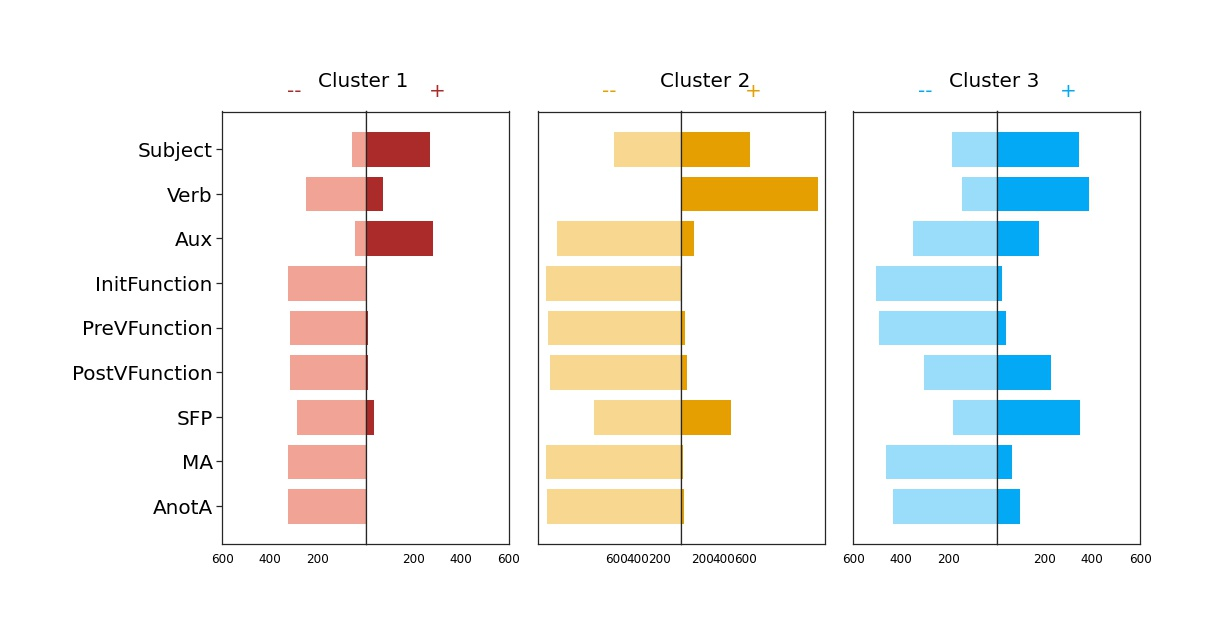
\includegraphics[width=1\textwidth]{figures/man-target-mid-syncluster.jpg}
    \caption{The number of sentences with/without a formal property in each cluster (Cluster 1 $\sim$ declaratives, Cluster 2 $\sim$ imperatives+declaratives, Cluster 3 $\sim$ interrogatives), darker colors represent the number of sentences with the property, lighter colors represent sentences without the property.}
    \label{fig:man-target-mid-syncluster}
\end{figure}

\bex{ex:mancl:midtarget:1}
\gll Zhe xia, (zhe shang).\\
This down (this up)\\
``This is down. (This is up)''
\eex

\subsubsection{Compare all four simulations}

Figure~\ref{fig:man-rand-compare-mid} compares the performance of all four simulations. We can see that the two \dlearnerabbr{} simulations are both bad at identifying clause types in Mandarin, but with pragmatics and some knowledge about A-not-A, the \plearnerabbr{} outperforms the other three models. 
\begin{figure}[H]
    \centering
    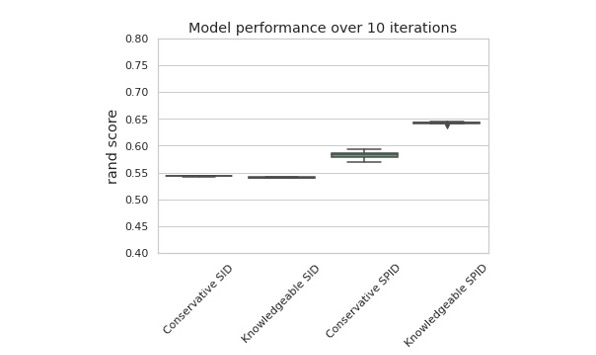
\includegraphics[width=1\textwidth]{figures/man-rand-compare-mid.jpg}
    \caption{Performance of conservative and knowledgeable \dlearnerabbr{} and \plearnerabbr{}}
    \label{fig:man-rand-compare-mid}
\end{figure}

Our results suggest that pragmatics is extremely crucial for Mandarin-acquiring children to identify clause types. Without pragmatics, learners might not be able to find any meaningful categories. Next, we are going to look at how much pragmatics the learners need.

\subsection{Simulations with noisy pragmatic information}
\label{sec:mancl:model:results:noisy}

Figure~\ref{fig:man-noisy-rand-cons} and \ref{fig:man-noisy-rand-mid} show the simulations with 0-100\% noise in the pragmatic information, as a conservative learner and a knowledgeable learner respectively. The performances of the \dlearnerabbr{} models are used as baselines and marked by the dotted line. As can be seen, the conservative \plearnerabbr{} model tolerates 20\% of noise in the pragmatics, and the knowledgeable model tolerates about 40\% of noise. Both are lower than the threshold for their English counterparts. This suggests that Mandarin learners rely heavily on the pragmatic information to identify clause type categories, as compared to their English counterparts. 

\begin{figure}[H]
    \centering
    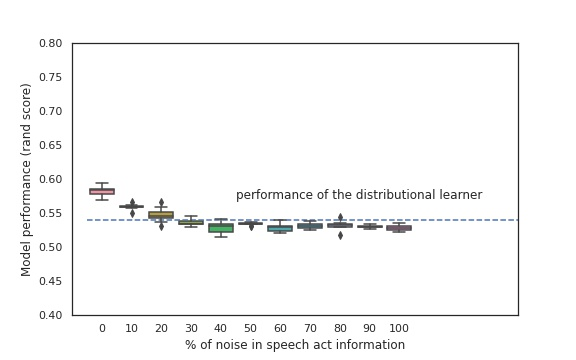
\includegraphics[width=1\textwidth]{figures/man-noisy-rand-cons}
    \caption{Performance of the conservative \plearnerabbr{} model with different levels of noise in the speech act information; dotted marks the rand score of the \dlearnerabbr{} learner}
    \label{fig:man-noisy-rand-cons}
\end{figure}

\begin{figure}[H]
    \centering
    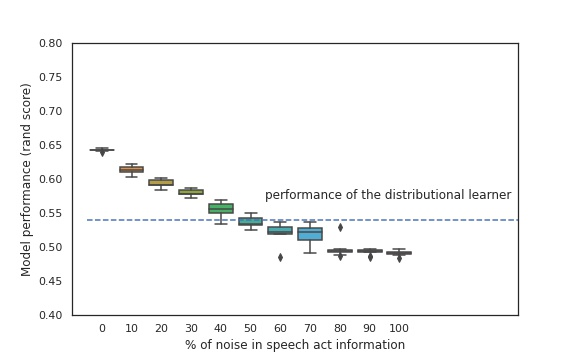
\includegraphics[width=1\textwidth]{figures/man-noisy-rand-mid}
    \caption{Performance of the knowledgeable \plearnerabbr{} model with different levels of noise in the speech act information; dotted marks the rand score of the \dlearnerabbr{} learner}
    \label{fig:man-noisy-rand-mid}
\end{figure}


\section{Discussion}
\label{sec:mancl:discussion}

In this chapter, we investigated how Mandarin-acquiring 18-month-olds can learn to identify the three clause types. As [+int] and [imp] in English and Mandarin are related to different surface features, comparing these two languages provides us with an opportunity to see the role of pragmatics in different languages.

Just like English parents, Mandarin parents also 
use clause types systematically, and the three clause types are predominantly mapped to their canonical functions (declaratives to assertions, interrogatives to questions, imperatives to requests/commands). The three clause types show distinctive formal profiles in the input available to children: compared to declaratives, interrogatives are more likely to have post-verbal UFIs, and more likely to have A-not-A and sentence final \tit{ma}; imperatives are more likely to not have subjects and negative modal \tit{bie}.

We then investigated the extent to which Mandarin learners need to rely on pragmatic information to identify clause types. I showed that, like in English, \dlearnerabbr{} simply cannot identify any of the right categories, even when we loosen our assumptions on learners' morpho-syntactic knowledge. But the \plearnerabbr{}, with pragmatic information, could identify all three clause types. Whereas a little pragmatics helps a lot for English learners, Mandarin learners require more accurate pragmatic information to succeed; when the noise in speech act exceeds 40 \% (20\% for learners with less morpho-syntactic knowledge), performance drops to the same level as syntax-only models.
Thus, pragmatics is essential for both English and Mandarin learners. But pragmatics is even more crucial for Mandarin learners, as the morpho-syntactic information is not enough for clause typing. 

So far, we have been just \emph{assuming} that children have access t, possibly very noisy, speech act information. As mentioned, this could lead to a chicken-and-egg problem: children need speech act to learn clause type, but at the same time they need clause type to learn speech act. In the next chapter, we explore other potential cues for pragmatic information that are not related to clause typing. As we have demonstrated with our simulations, learners of both English and Mandarin can tolerate some noise in the pragmatic information used to infer clause type. If cues other than clause type (e.g. parents' attention behavior) are informative of speech act to some extent, this may already be sufficient to solve the clustering problem of clause typing. In the next chapter, we specifically look at three such cues, prosody, speech gaps, and parents' attention.

